\documentclass[12pt]{article}

% Page formatting. 
\usepackage[a4paper,top=2cm,bottom=2cm,left=2cm,right=2cm,marginparwidth=1.75cm]{geometry}
\usepackage[parfill]{parskip}

% Typesetting for mathematics.
\usepackage{amsmath,amsthm,amssymb}
\usepackage{tikz-cd}

% Image Formatting
\usepackage{graphicx}
\usepackage{pdfpages}
\usepackage{subfig}

%============================================================================================================================
 
\title{\vspace{-4ex} Kinetic-Sunyaev Zoldovich Effect \vspace{-1ex}} 
\author{Advisor: Dr. Cooney \\
Author: \underline{Jesse Randall}\vspace{-2ex} \\
}  
 
\begin{document}

\maketitle

\section{Introduction}

The early universe was a soup of ions and high energy photons due to the high temperatures and density of matter. The black body spectrum of matter at these high temperatures says that the average energy of photons being emitted would have been high enough to ionize any atoms that formed. Therefore the early universe was opaque to photons as they had a relatively short mean free path. After a period of expansion and cooling, the era of recombination occurred where the photons being produced were not as energetic allowing the formation of atoms. This allowed the transmission of photons and so the universe became transparent for the first time. 

We see this primordial radiation today as the Cosmic Microwave Background. (CMB) The CMB is a remnant of the early universe and contains a lot of useful information about the state of the early universe. The photons we receive from the CMB give us a map of the surface of last scattering through the tiny differences in their wavelengths known as anisotropies. Photons of shorter wavelength left an area of lower density while photons of longer wavelength left an area of higher density. From these anisotropies in the CMB we effectively have a map of the relative distribution of matter in the early universe.

This project is focused on calculating the anisotropies in the CMB produced by the kinetic Sunyaev-Zoldovich effect (KSZ) as a way to quantify to the effect that rotational velocities have on the scattering of the CMB. This effect occurs when photons from the CMB are scattered by the collapsed matter between the observer and the surface of last scattering (SOLS). Dr. Cooney has already performed these calculations for his dissertation and so I was tasked with checking his work while being more careful to avoid and catch any mistakes he may have made.

We have decided to use the Python programming language for all calculations as I have a lot of experience using it through the classes I have taken, and it provides some modules that make the coding much easier to write as well as read.

\section{Power Spectrum}

The work I have done thus far has been to reproduce the results of Dr. Cooney’s dissertation found in Chapter 5. It focuses on the ingredients necessary to calculate the KSZ angular power spectrum. This is needed for the modeling of the distribution of matter in the universe so that we can get a statistical average of the amount of matter that a photon would encounter along its path from the SOLS to the Earth. The distribution of matter is believed to be heavily affected by dark matter as well as most galaxies we have observed appear to rotate much faster than anticipated with the amount of visible matter measured. This is explained by the presence of dark matter halos that provide the unforeseen mass needed for the observed rotational velocities. Therefore later on we will discuss the statistical distribution of dark matter halos and how they affect the clustering of matter as well.

First task was to graph the dimensionless linear order density-density power spectrum (LPS) of matter which gives a statistical measure of gravitational clustering. The model used is given by Ma (1998) and shown in equation (\ref{lps}).
\begin{equation} \label{lps}
P(k,a) = \frac{Ak^n [D(a) / D_0]^2 [ln(1+\alpha_1 q) / \alpha_1 q]^2}{[1 + \alpha_2q + (\alpha_3 q)^2 + (\alpha_4 q)^3 + (\alpha_5 q)^4]^{1/2}}
\end{equation} 

It is a function of the wavenumber $k (Mpc^{-1})$, the spatial frequency of a wave, and the scale factor $a$, the dimensionless parameter used to characterize the relative expansion of space. $n$ is the spectral index and $n \approx 1$ for the scales we are considering. The constants $\alpha_i$ are numerical constants found through N-body simulations. The dimensionless LPS (DLPS) is given below in equation (\ref{dlps}).
\begin{equation} \label{dlps}
\delta_t(k) = \frac{1}{(2\pi)^3} \frac{k^3 P(k)}{2\pi^2}
\end{equation}

Some issues were encountered due to a normalization factor being left out in the description of what was being graphed underneath the figure. However, after adding it my results matched and are plotted in Figure (\ref{dlpsFig}).

\begin{figure}[!ht]
    \centering
    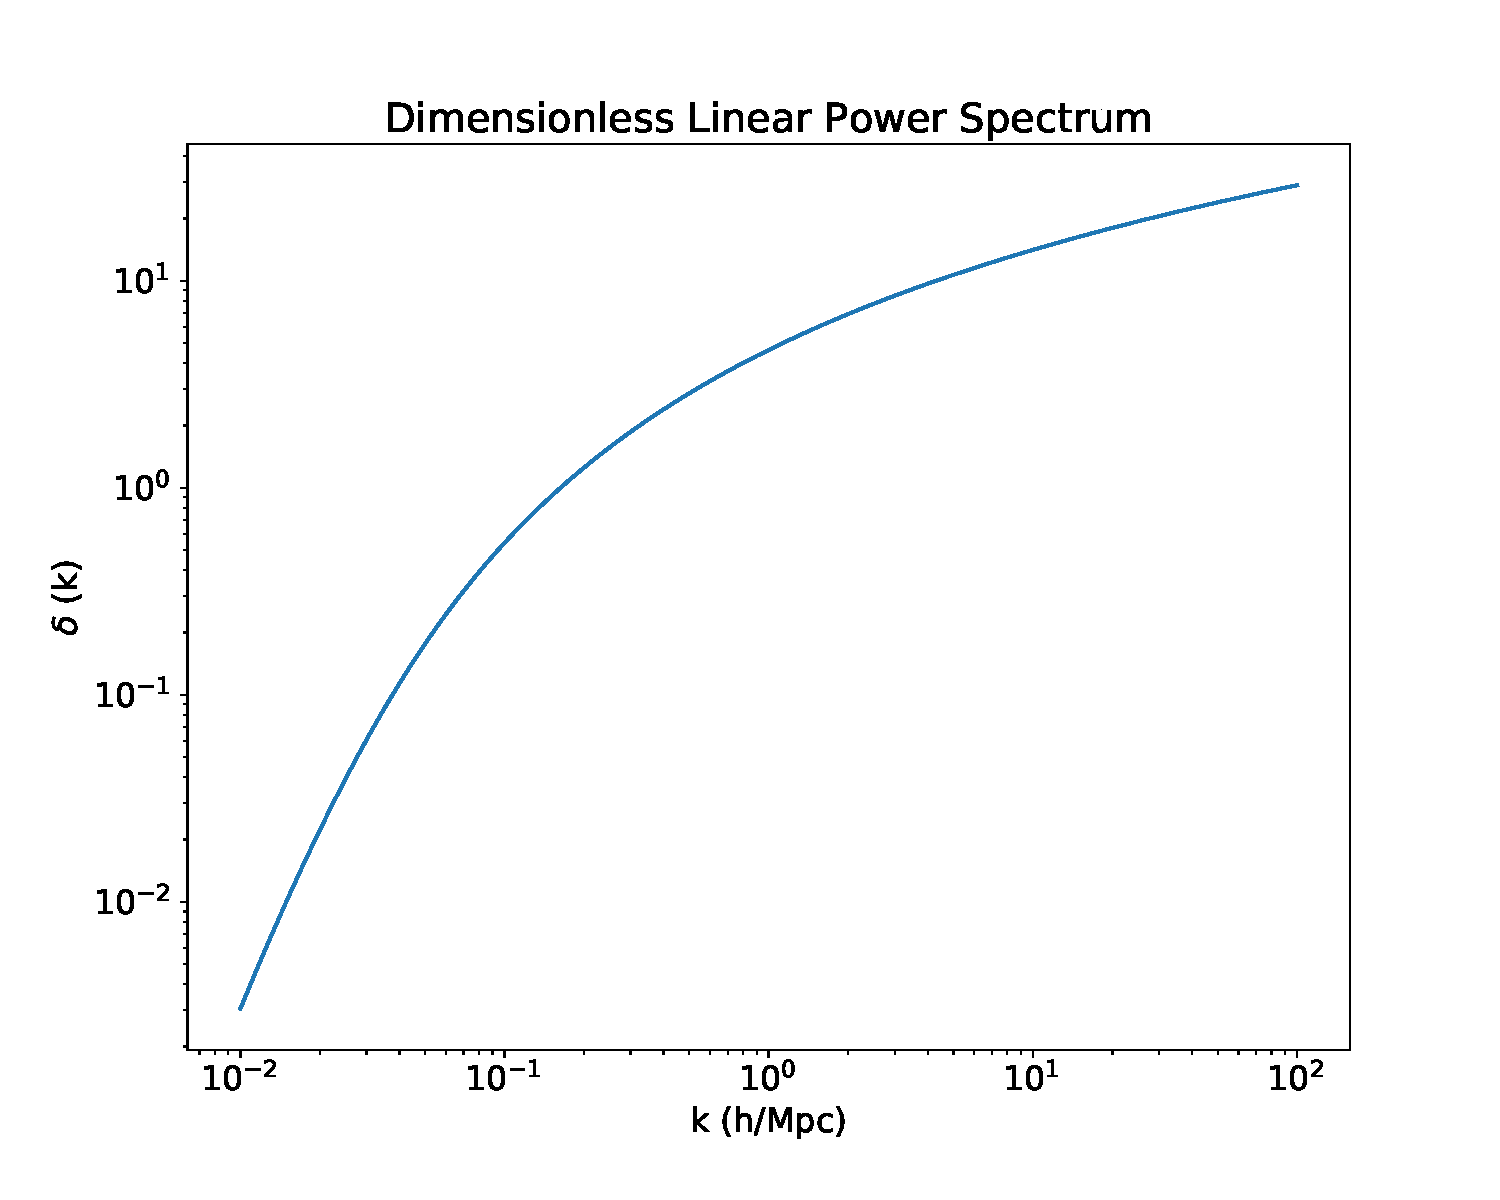
\includegraphics[width=0.8\linewidth,keepaspectratio=false]{figures/DLPS.pdf}
    \caption{Plot of the Dimensionless Linear Power Spectrum used in upcoming calculations.}
    \label{dlpsFig}
\end{figure}

My next task was to plot the standard deviation of the density contrast which is needed for the analysis of the Press-Schechter  and Sheth-Tormen mass functions. Equation (\ref{varR}) is the variance and you can obtain the standard deviation by taking the square root.
\begin{equation} \label{varR}
\sigma^2(R) = \int_{0}^{\infty} \frac{4 \pi k^2}{(2 \pi)^3} P(k) \tilde{W}^2(kR) dk
\end{equation}
It is a function of the radius of the sphere that we are observing. However, it is being plotted as a function of the mass contained within the sphere of interest so a substitution is made of the form $M = 4 \pi \rho_0 R^3 / 3$.
\begin{equation} \label{varM}
\sigma^2(M) = \int_{0}^{\infty} \frac{4 \pi k^2}{(2 \pi)^3} P(k) \tilde{W}^2(kM) dk
\end{equation} 
It consists of the LPS from before and the fourier transform of the top hat window function given in equation (\ref{thwf}).
\begin{equation}\label{thwf}
\tilde{W}(x) = \frac{3(sin(x) - xcos(x))}{x^3}
\end{equation}
The top hat window function has the value one inside the sphere we are observing and zero everywhere else. This removes the need to worry about fluctuations outside the region of interest.

Performing this calculation requires numerical integration so as a first step Dr. Cooney recommended plotting the integrand to see if it has any irregularities. Figure (\ref{intFig}) shows that for $k > 1$ for low values of $M$ produces high frequency oscillation in the integrand which is not handled well by normal numerical integration. This trend is shown to continue towards lower values of $k$ with increasing $M$. It would require special numerical techniques to evaluate the integral with reasonable error. However, the oscillations start to occur after the integrand has decreased by several orders of magnitude leading to a minimal contribution to the value of the integral for large values of $k$. Therefore an approximation is used by evaluating the integral up to a certain value of $k$ instead of the entire range of the limit of integration. This avoids the issues caused due to the oscillations while still retaining major contribution to the integral.

\begin{figure}[!ht]
    \centering
    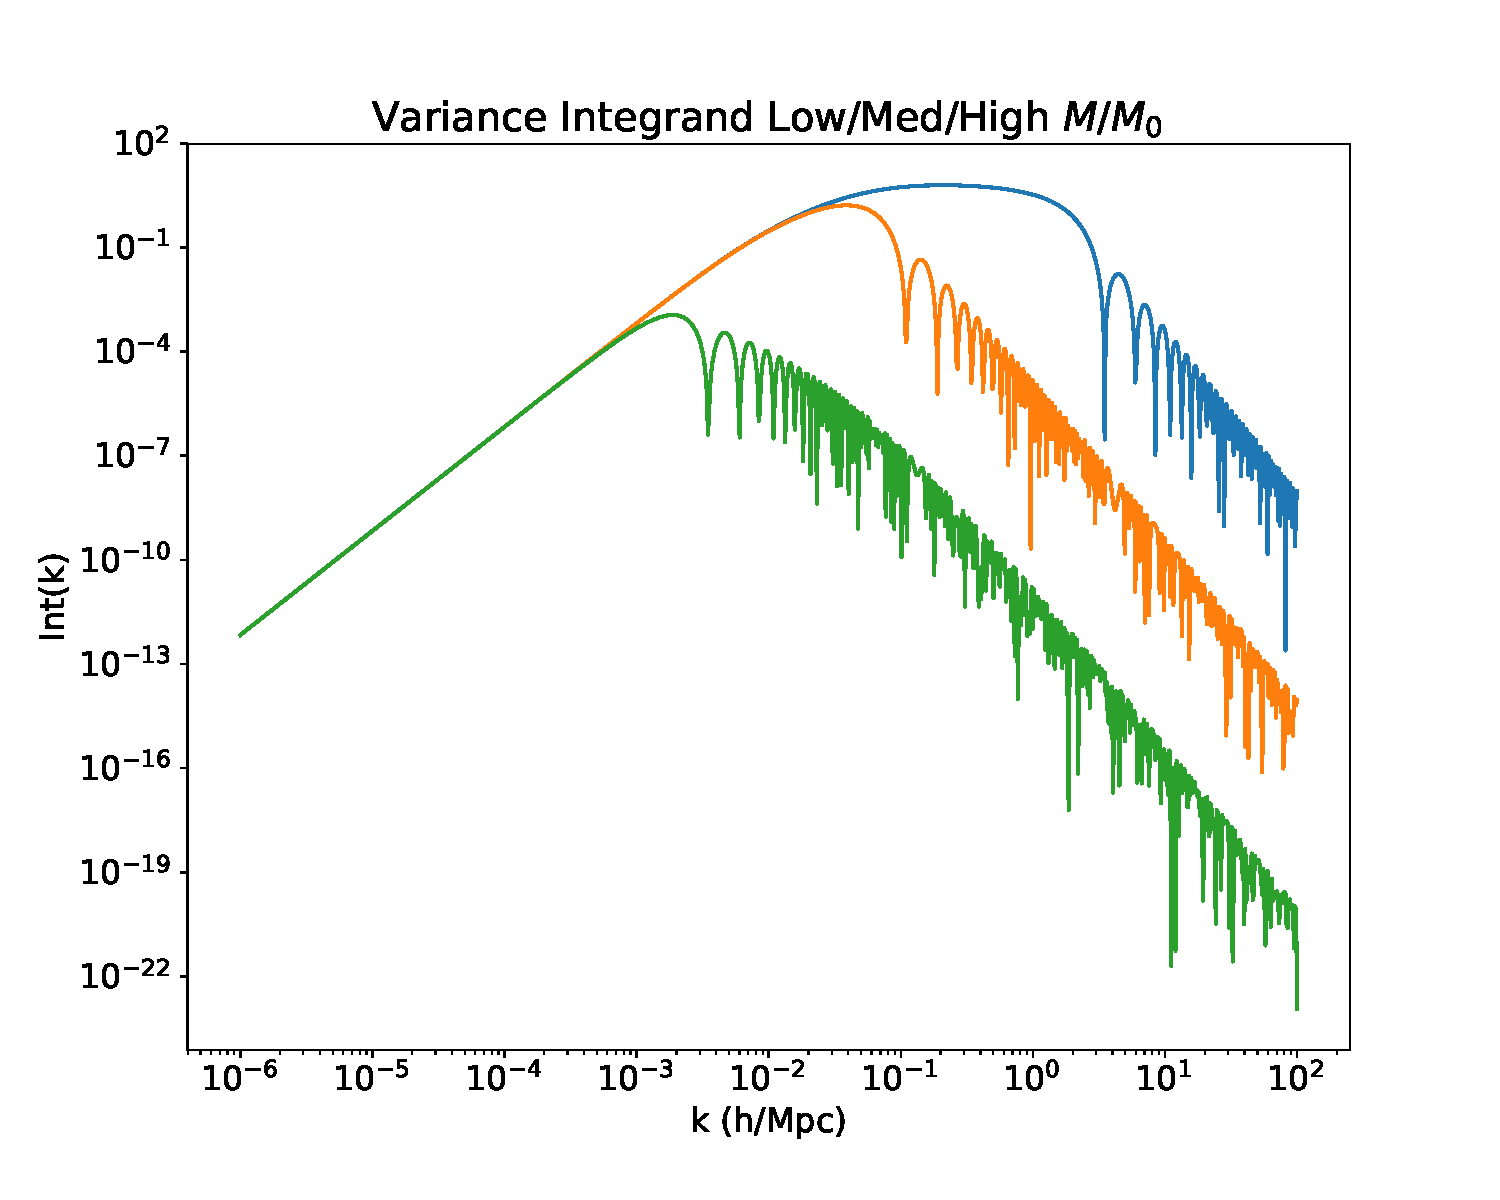
\includegraphics[width=0.8\linewidth,keepaspectratio=false]{figures/VARIntALL.pdf}
    \caption{Plots of the integrand of the variance over a range of M values to get a quantitative picture of its behavior. Low M plotted in blue, medium M plotted in orange, and high M plotted in green.}
    \label{intFig}
\end{figure}

Again issues with normalization were encountered causing the standard deviation that I was calculating to be several orders of magnitude lower than the values shown in Dr. Cooney's dissertation. By removing the normalization term that was added previously to the DLPS my results matched and are plotted in Figure (\ref{stdFig}). I anticipate that further normalization issues may arise and so I will look into which approach is correct if further inconsistencies arise.

\begin{figure}[!ht]
    \centering
    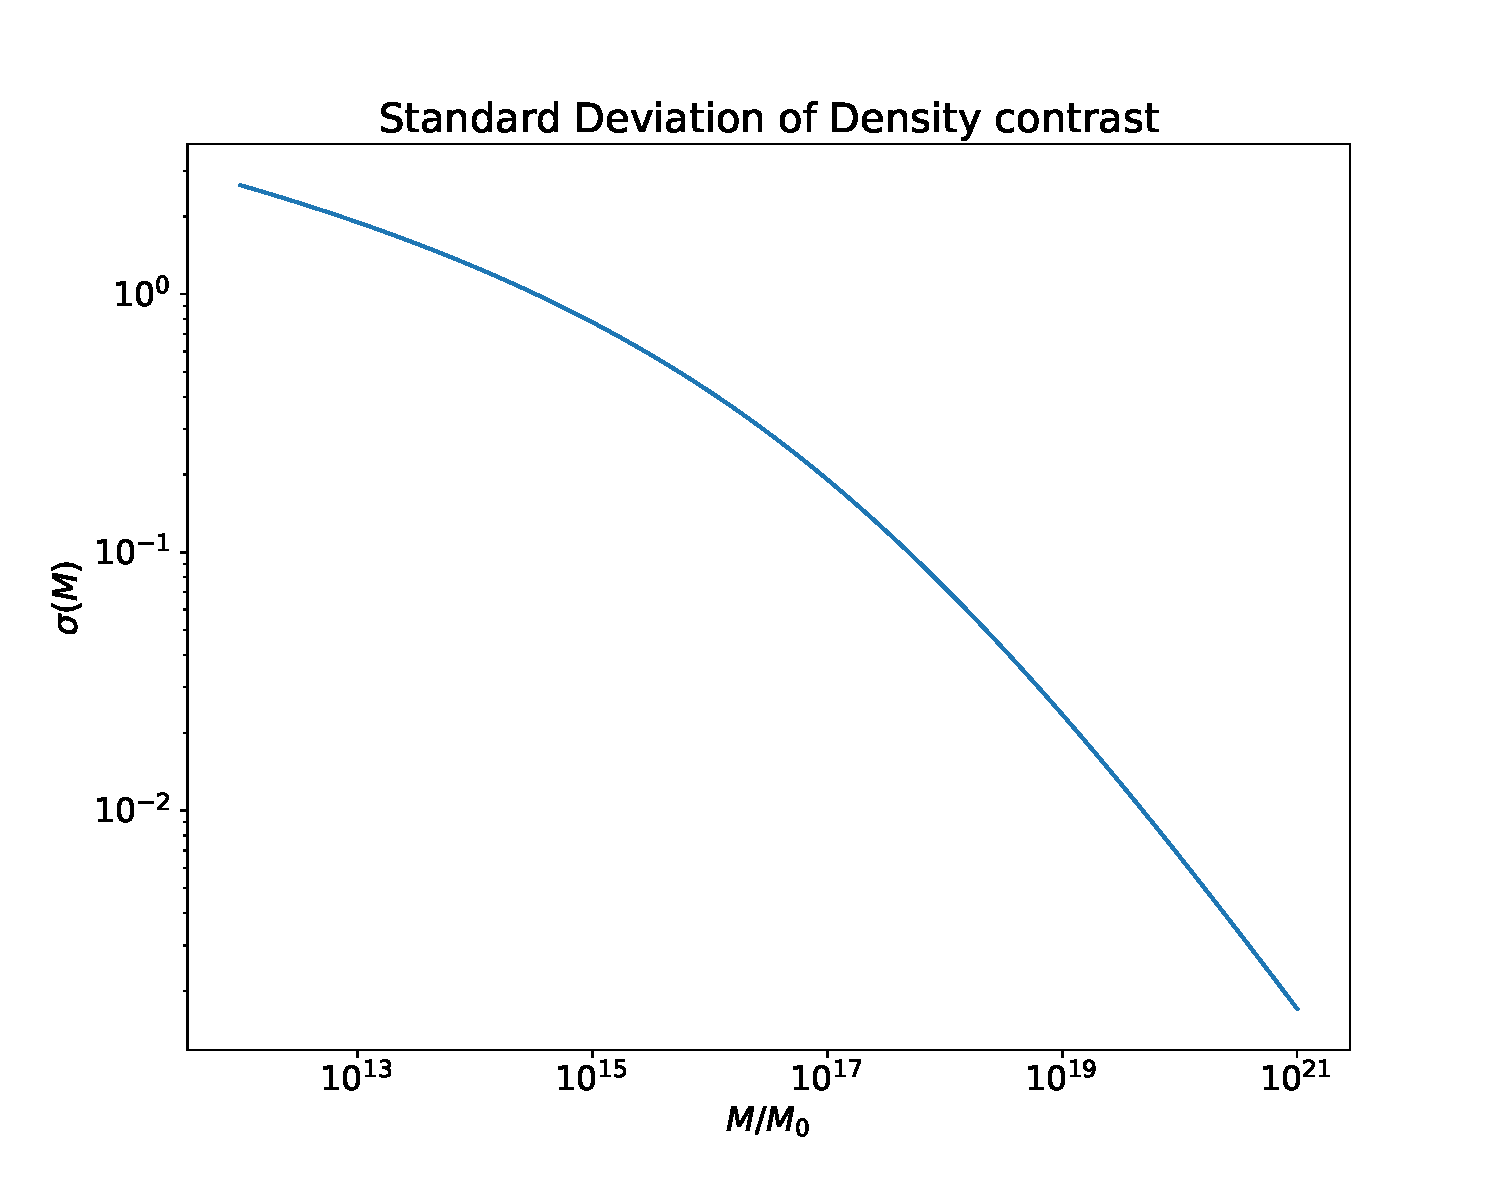
\includegraphics[width=0.8\linewidth,keepaspectratio=false]{figures/SD.pdf}
    \caption{Plot of the standard deviation of the density contrast.}
    \label{stdFig}
\end{figure}

My next task was to determine the importance of the bias factor $b(M)$ given by Jing (1998) found in the power spectrum we are constructing and whether or not simulations with greater accuracy have been performed since to improve it.
\begin{equation}
b(M) = \Big (1 + \frac{\nu^2 - 1}{\delta_c} \Big ) \Big (\frac{1}{2\nu^4} + 1 \Big )^{0.06-0.02n}
\end{equation}
Mo and White (1996) provided the analytical model for the derivation of the first part of the bias factor. Jing (1998) improved it to match their N-body results for $M < M_*$ ($M_*$ is the characteristic nonlinear mass scale defined by $\nu(M_*) =  1$) as there was significant disagreement so the second half of the bias factor was added. The bias factor gives the relationship between the spatial distribution of galaxies and the underlying dark matter density field, and is plotted in Figure (\ref{biasFig}).

\begin{figure}[!ht]
    \centering
    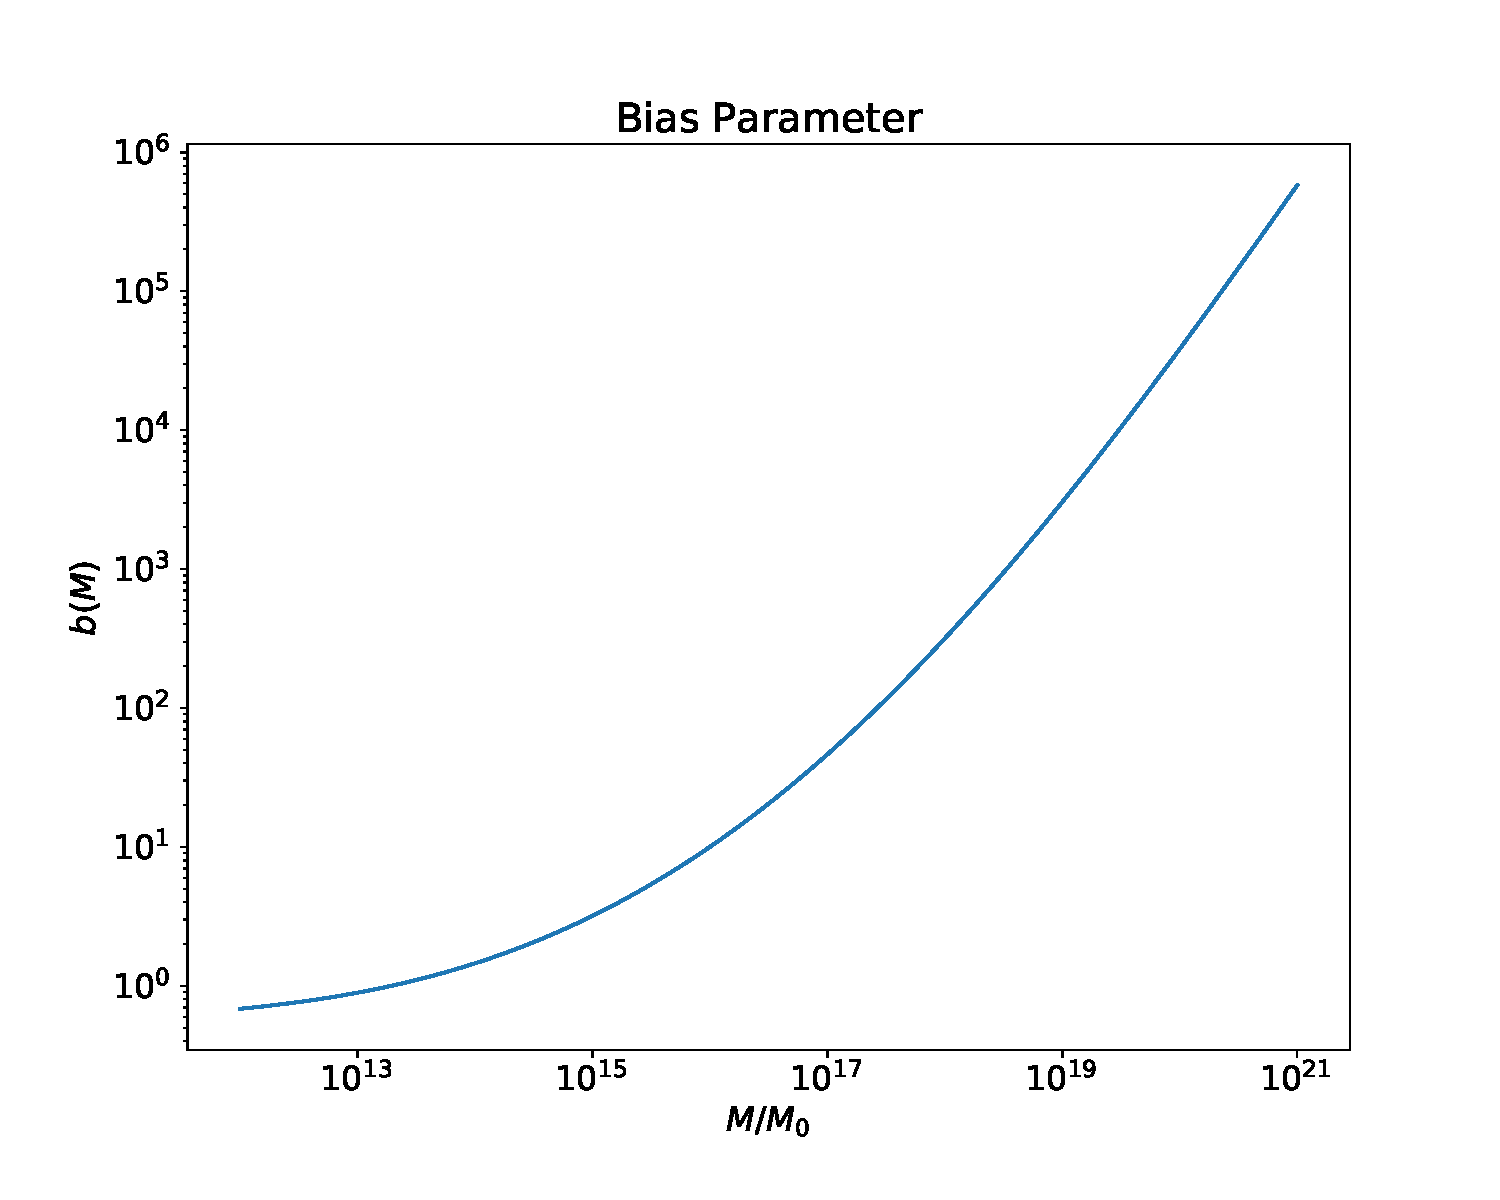
\includegraphics[width=0.8\linewidth,keepaspectratio=false]{figures/BIAS.pdf}
    \caption{Plot of the bias factor.}
    \label{biasFig}
\end{figure}

I encountered a discrepancy between Mo and White (1996) and Jing (1998) when determining the purpose of the bias factor and would like to make note of it. The term $\nu$ in the bias factor from Jing (1998) is defined as $\nu(M) \equiv \delta_c / \sigma(M)$ and referenced as the peak height. $\delta_c$ is used when defining the redshift at which a spherical perturbation of linear overdensity $\delta$ collapses in an Einstein de Sitter universe given by $z_c = \delta / \delta_c - 1$  with $\delta_c = 1.68$. However, in Mo and White (1996) the bias factor is defined as
\begin{equation} \label{MWbf}
b(M) = \Big (1 + \frac{\nu_1^2 - 1}{\delta_1} \Big )
\end{equation}
with $\nu_1 \equiv \delta_1 / \sigma_1(M)$ and $\delta_1 \equiv (1 + z_1)\delta_c$. The reason there is this difference is that Mo and White (1996) use the "values linearly extrapolated to the present time" (justified as '$\delta$ and $\sigma$ grow with time in the same manner in linear perturbation thory, it is convenient to use their values linearly extrapolated to the present time') and the subscripts denote the smoothing radius for the sphere of interest [$\sigma_1 = \sigma(R_1), \delta_1 = \delta(R_1)$]. Therefore Mo and White (1996) are looking at the collapsed spherical overdensity while Jing (1998) is looking at the uncollapsed spherical overdensity.

From this the power spectrum is the sum of two contributions, a one-halo term and a halo-halo term given below in equations (\ref{1h}) and (\ref{2h}) respectively.
\begin{equation} \label{1h}
P_{1h}(k) = \int dM \frac{dn}{dM} [r_{s}^3 \delta_a \bar{u} (kr_s)]^2
\end{equation}
\begin{equation} \label{2h}
P_{2h}(k) = \Big [ \int dM \frac{dn}{dM} r_{s}^3 \delta_a \bar{u} (kr_s) b(M) \Big ]^2 P_{lin}(k)
\end{equation}
We shall break down each term of these contributions to better understand where they come from. All calculations can be found in Ma and Fry (2000). First, n is the number density of dark matter halos in a spherical region of a given radius. We can write it as a function of mass using the equation for the density of a sphere. Then taking its derivative with respect to the amount of mass contained in the spherical region gives us the mass function, $dn/dM$. Sheth-Tormen improved upon the original Press-Schecter mass function by fitting to N-body simulations, found in equation (\ref{STMF}).
\begin{equation} \label{STMF}
\frac{dn}{dlnM} = \frac{\rho_{0}}{M} \frac{d ln \sigma^{-1}}{d ln M} 2A  \Big (1 + \frac{1}{\nu'^{2q}} \Big) \Big(\frac{\nu'^{2}}{2 \pi} \Big)^{1/2} e^{-\nu'^{2} / 2}
\end{equation}
The numerical constants are $\alpha = 0.707$, $q = 0.3$ and $A = 0.322$ where $\nu' = \alpha^{-1/2} \nu$. The scale radius, $r_s$, is the next term and is found in equation (\ref{SR}).
\begin{equation} \label{SR}
R_s = \frac{R_{200}}{c} = \frac{1}{c} \Big(\frac{3M}{800\pi\rho_0}\Big)^{1/3}
\end{equation}
$R_{200}$ is the radius within which the average density is 200 times the mean density of the universe. Therefore it is related to the mass contained in this region by $M = 800\pi\rho_{0}R_{200}^{3}/3$. $c$ is the concentration parameter and is given by equation (\ref{CP}).
\begin{equation} \label{CP}
	c(M) = 
	\begin{cases}
		5\sigma(M) & M/M_0 < 10^{14} \\
		9\sigma(M) & M/M_0 > 10^{14} \\
	\end{cases}
\end{equation}
Next the density amplitude, $\delta_a$, is given by equation (\ref{DA}).
\begin{equation} \label{DA}
	\delta_a(M) = 
	\begin{cases}
		\frac{200c^{3}}{3[ln(1+c) - c/(1+c)]} & M/M_0 < 10^{14} \\
		\frac{100c^{3}}{ln(1+c^{3/2})} & M/M_0 > 10^{14}
	\end{cases}
\end{equation}
Finally, we have the Fourier-transform of the density profile, $\tilde{u}(kr_{s})$. In the calculations we used a mixed profile density that uses NFW for $M/M_0 < 10^{14}$ and Moore for $M/M_0 > 10^{14}$.
\begin{equation} \label{DP}
	\tilde{u}(q) = 
	\begin{cases}
		\frac{4\pi\{ln(e+1/q)-ln[ln(e+1/q)]/3\}}{(1+q^{1.1})^{(2/1.1)}} &  M/M_0 < 10^{14} \\
		\frac{4\pi\{ln(e+1/q)+0.25ln[ln(e+1/q)]\}}{1+0.8q^{1.5}} &  M/M_0 > 10^{14} \\
	\end{cases}
\end{equation}
Issues with differentiation arose due to the roundoff error present in numerical calculations. I am using the method scipy.misc.derivative in the Scipy package for Python. It uses a third order finite difference method which is based on the definition of the of derivative through the limit process which requires the step size $dx \ll 1$. However, the point that I am taking the derivative at has a magnitude in the range $10^{40}-10^{50}$. When subtracting dx from such a large number it cannot account for that level of precision and the result of the difference is just the point that I am evaluating at due to roundoff. A detailed analysis of the algorithm being used is given in the next section.

\section{Power Spectrum Algorithm}

This is a detailed analysis of the algorithm used to calculate the integrand of the one halo power spectrum contribution given in equation (\ref{INT}). 
\begin{equation} \label{INT}
    P_{1h,Int}(M, k) = \frac{dn}{dM} [r_{s}(M)^3 \delta_a(M) \bar{u} (kr_s)]^2
\end{equation}
The function is initially called with the first argument being a 64-bit floating point number for the mass $M$ in units of $kg$ and the second argument being a 64-bit floating point number for the wavenumber $k$ in units of $Mpc^{-1}$. First, the concentration parameter $c(M)$ is called, given in equation (\ref{CP}), to reduce the number of function calls in following calculations. 
\begin{equation} \label{CP}
	c(M) = 
	\begin{cases}
		5\sigma(M) & M/M_0 < 10^{14} \\
		9\sigma(M) & M/M_0 \geq 10^{14} \\
	\end{cases}
\end{equation}
It is defined piece-wise such that for $M/M_\odot < 10^{14}$ then $5\sigma(M)$ is returned, else if $M/M_\odot \geq 10^{14}$ $9\sigma(M)$ is returned and stored as the variable $cp$. Next, the scale radius $r_s(M)$ is called and is given in equation (\ref{SR}).
\begin{equation} \label{SR}
    r_s(M) = \frac{1}{c(M)} \Big(\frac{3M}{800 \pi \rho_0} \Big)^{1/3}
\end{equation}
It takes the parameters $M$ and $cp$. The mean density of the universe $\rho_0$ has units of $kg / m^3$ so $r_s$ returns a value with units of meters and is stored in the variable $sr$. The next function we will observe is for $\delta_a(M)$ which is given in equation (\ref{DA}).
\begin{equation} \label{DA}
	\delta_a(M) = 
	\begin{cases}
		200c^{3} / 3[ln(1+c) - c/(1+c)] & M/M_0 < 10^{14} \\
		100c^{3} / ln(1+c^{3/2})        & M/M_0 \geq 10^{14}
	\end{cases}
\end{equation}
It takes parameters $M$ and $cp$. Similar to the function for the concentration parameter, if  $M/M_\odot < 10^{14}$ then the delta function for the NFW profile is returned, else if  $M/M_\odot \geq 10^{14}$ then the delta function for the Moore profile is returned. Next we will look at the function for the Fourier transform of the mixed density profile $\bar{\mu}(kr_s)$ found in equation (\ref{DP}). It uses the algebraic expressions found in Ma and Fry (2000). 
\begin{equation} \label{DP}
	\bar{\mu}(q) =
	\begin{cases}
		4\pi\{ln(e+1/q)-ln[ln(e+1/q)]/3\} / (1+q^{1.1})^{(2/1.1)} & M/M_0 < 10^{14} \\
		4\pi\{ln(e+1/q)+0.25ln[ln(e+1/q)]\} / (1+0.8q^{1.5})      & M/M_0 \geq 10^{14}
	\end{cases}
\end{equation}
It takes the parameters $k$, converted to $m^{-1}$, multiplied by $rs$ and $M$. Again, if $M/M_\odot < 10^{14}$ then the density profile for the NFW profile is returned, else if  $M/M_\odot \geq 10^{14}$ then the density profile for the Moore profile is returned. Then the results of those functions are multiplied together as shown in the parentheses and squared.

Next function is the Sheth-Tormen mass function $dn/dM$ found in equation (\ref{STM}).
\begin{equation} \label{STM}
	\frac{dn}{dM} = \frac{1}{M} \frac{dn}{dlnM} = \frac{\rho_{0}}{M} \frac{d ln \sigma^{-1}}{dM} 2A  \Big (1 + \frac{1}{\nu'^{2q}} \Big) \Big(\frac{\nu'^{2}}{2 \pi} \Big)^{1/2} e^{-\nu'^{2} / 2}
\end{equation}

Issues with differentiation of $\frac{d ln \sigma^{-1}}{dM}$ arose due to the limited precision in numerical calculations. I am using the method scipy.misc.derivative in the Scipy package for Python. It uses a third order finite difference method found in equation (\ref{FDM}).
\begin{equation} \label{FDM}
	f'(x) \approx \frac{f(x+dx) - f(x-dx)}{2dx}
\end{equation} 
It is based on the definition of the derivative through the limit process which requires the step size $dx \ll 1$. However, the point that I am taking the derivative at has a magnitude in the range $10^{40}-10^{50}$. Unfortunately, 64-bit floating point numbers have a precision of 15 significant figures. Therefore the addition and subtraction of numbers that have a greater difference than 15 orders of magnitude cannot be performed.

\end{document}